\documentclass[12pt]{article}
\usepackage[utf8]{inputenc}
\usepackage[acronym, toc]{glossaries}
\usepackage{amsmath}
\usepackage{amssymb,amsfonts,latexsym,cancel}
\usepackage{graphicx}
\usepackage{float}
\usepackage{subfig}
\usepackage[normalem]{ulem}
\usepackage[lmargin=3cm,rmargin=3cm,top=2.5cm,bottom=2.5cm]{geometry}
\usepackage{longtable}
\usepackage{ragged2e}
\usepackage{datetime}
\usepackage{parskip}
\usepackage{fancyhdr}
\usepackage{titling}
\pagestyle{fancy}
\setlength{\headheight}{15.71667pt}
\usepackage{hyperref}
\hypersetup{
    colorlinks,
    citecolor=black,
    filecolor=black,
    linkcolor=black,
    urlcolor=black
}

\usepackage[
  backend=bibtex,
  style=ieee,
  url=false,
  doi=true,
  isbn=false
]{biblatex}
\addbibresource{bibliography.bib}


\lhead{}
\rhead{}

\fancyfoot{}
\renewcommand{\footrulewidth}{0.5pt}
\fancyfoot[R]{\thepage}

\title{ NON-Textual Data Extraction % Título de la práctica
}
\author{ Sergio Marín Sánchez % Nombre del autor
}
\newdate{date}{26}{2}{2024} % Fecha

\begin{document}
\begin{titlepage}
    \centering
    \phantom{a}
    \vspace{1cm}
    {
\includegraphics{ESCUDO_UPM.pdf}\par}
    \vspace{1cm}
    {\bfseries\LARGE Universidad Politécnica de Madrid \par}
    \vspace{1cm}
    {\scshape\Large Escuela Técnica Superior de Ingenieros Informáticos \par}
    \vspace{1cm}
    {\scshape\Huge \thetitle \par}
    \vfill
    {\itshape\large Authors: % Nombre del Profesor
     \par}
    {\large \theauthor \par}
    {\large Irune Monreal Iraceburu \par}
    {\large Ander Ros Ollo \par}
    \vspace{0.2cm}
    {\large Date: \displaydate{date} \par}
\end{titlepage}

\section{Motivation}

The implementation of Content-Based Image Retrieval (CBIR) in the field of poker cards offers a practical application in the world of entertainment and gaming. For example, in online gaming platforms or poker applications, CBIR can be used to enhance the user experience by allowing them to quickly find poker cards similar to those they wish to purchase or collect. Users could upload an image of a specific card they are looking for, and the system would show them similar options available on the platform. This streamlines players' card search and acquisition process, thus increasing their satisfaction and engagement on the platform. In addition, CBIR can be applied in training applications or poker tutorials to quickly identify specific cards during practice, thus helping players improve their skills and understanding of the game.

\section{State of the art}

In our project development, we have relied on the research paper titled \textit{Comparative study of histogram distance measures for re-identification}\cite{marin-reyes_comparative_2016} and a couple of online resources that helped demystify the inner workings of \textit{Harris Corner and Edge Detector}\cite{berrios_harris_2024} and \textit{Histogram of Oriented Gradients explained using OpenCV}\cite{noauthor_histogram_2016}.

The paper emphasized the importance of histogram binning, cautioning against an excessive number of bins due to potential noise and computational overhead, especially in images with limited color ranges. Taking this into consideration, we opted for a binned histogram approach to ensure consistent treatment of similar colors, yielding promising results while keeping computational costs low.

\begin{figure}[H]
    \centering
    
\includegraphics[width=0.5\textwidth]{imgs/histogram.png}
\end{figure}

When it came to selecting a distance measure for histograms, we landed on Chi-Square for its solid statistical foundation and manageable computational complexity, aligning with the paper's findings of its effectiveness.

\begin{equation*}
    d_{\chi^2}(x, y) = \frac{1}{2}\sum_{i = 1}^n \frac{\left(x_i - y_i\right)^2}{x_i + y_i}
\end{equation*}

Additionally, the paper highlighted the benefits of segmenting images into stripes for improved re-identification accuracy. Following this advice, we divided our images into a 4x5 grid, assigning varying weights to different regions, with particular emphasis on central stripes and specific corners to enhance signal clarity amidst noise.

In fine-tuning the parameters of the Harris Corner and edge detector, we opted to increase sensitivity by adjusting the k parameter. Similarly, for HOG analysis, we configured the window size to encompass the entire image while setting a smaller cell size, mirroring the approach taken with the histogram descriptor, to focus on finer details, inside the card.

Moreover, we conducted extensive experimentation by exploring different combinations of descriptors. Specifically, we experimented with three distinct approaches: a weighted combination of histogram and HOG descriptors, prioritizing the ranking of images based on the histogram descriptor followed by the top 20 ranked images based on the HOG descriptor, and conversely, prioritizing the ranking based on the HOG descriptor followed by the top 20 ranked images based on the histogram descriptor. By exploring these variations, we sought to uncover the most effective fusion strategy to enhance the accuracy and robustness of our re-identification system.

By integrating insights from academic research with practical experimentation, our project aims to advance re-identification methodologies, offering both efficiency and effectiveness in our real-world application.

\section{Implementation of the toy CBIR}

\subsection{A `smart' histogram descriptor + distance}

In the pursuit of a tangible implementation, the chosen approach involves a 'smart' histogram descriptor coupled with an effective distance metric. The smart histogram descriptor aims to capture intricate visual features of poker cards, considering color distribution and intensity variations. The chosen distance metric ensures that the retrieval system can effectively discern similarities and differences between images.

\begin{figure}[H]
    \centering
    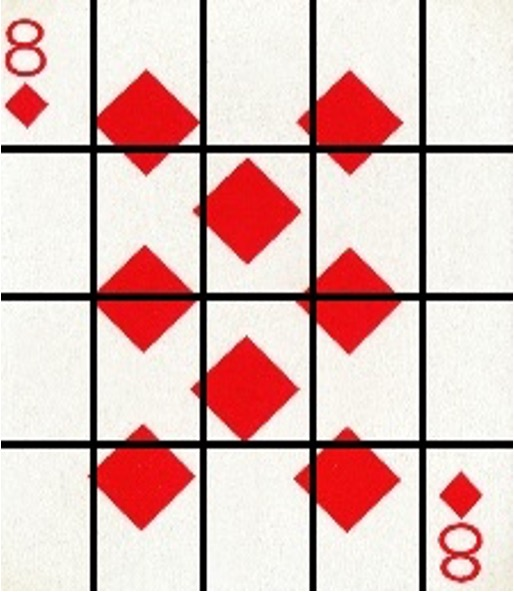
\includegraphics[width=0.25\textwidth]{imgs/sub_images.jpg}
\end{figure}

To elaborate on our implementation, we have divided the images into a $5 \times 4$ grid to better capture and represent their figures along with their respective colors. Our emphasis is on assigning higher weights to the central six grids, as these regions are deemed more crucial in terms of color relevance for distinguishing between cards. An exception to this weighting scheme is observed in the card representing the number `2' where the absence of significant features in the center justifies a different approach.

We have categorized the weights into three levels: the central six grids, corners (top-left and bottom-right), and edges. The weights for the central six grids are evenly distributed with a weight of 0.1 each. The corners, representing the top-left and bottom-right regions, carry a weight of 0.15 each. The remaining grids, encompassing the edges, are assigned a weight of 0.083 each. This meticulous weighting strategy aims to ensure that the descriptor captures and prioritizes the most distinguishing features of poker cards, enhancing the effectiveness of our content-based image retrieval system. 

The image shown below displays its top five visually similar counterparts, based on the distances calculated using the smart histogram descriptor.

\begin{figure}[H]
    \centering
    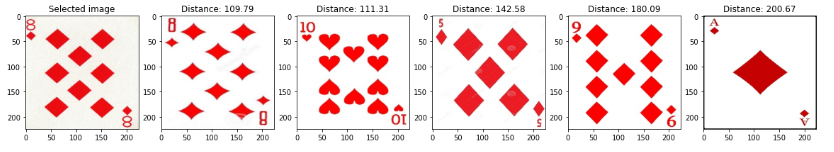
\includegraphics[width=\textwidth]{imgs/hist_order.png}
\end{figure}

\subsection{An additional descriptor + distance, eg: Harris + HOG + $\chi^2$ distance}

To further augment the CBIR capabilities, an additional descriptor in the form of Harris corners and Histogram of Oriented Gradients (HOG) is introduced. The Harris corners highlight key interest points, while HOG captures shape and edge information. The Chi-square distance metric is then applied to quantify the dissimilarity between the reference image and each image in the dataset.

In fine-tuning the parameters of the Harris Corner and edge detector, we opted to increase sensitivity by adjusting the \texttt{k} parameter. Similarly, for HOG analysis, we configured the window size to encompass the entire image while setting a smaller cell size ($56 \times 45$ pixels) to focus on finer details, mirroring the approach taken with the histogram descriptor.

The image shown below displays its top five visually similar counterparts, based on the distances calculated using the combination of Harris + HOG descriptors

\begin{figure}[H]
    \centering
    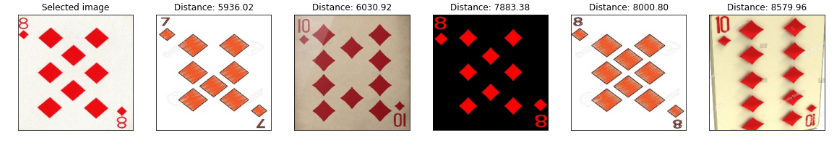
\includegraphics[width=\textwidth]{imgs/hog_order.png}
\end{figure}

\subsection{How to combine both descriptors}

We experimented with three distinct approaches to combine both descriptors: 

\begin{itemize}
    \item A weighted combination of the histogram and HOG descriptors, where their flattened feature vectors are combined into a unified one, giving 30\% importance to the histogram descriptor and 70\% to the HOG one. This combined feature vector serves as the basis for distance calculations during retrieval
    \begin{figure}[H]
        \centering
        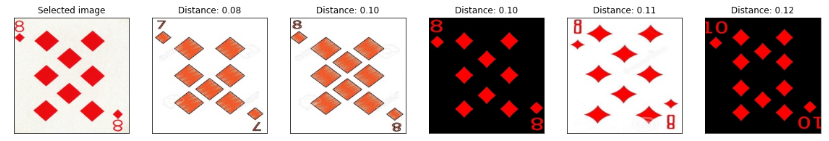
\includegraphics[width=\textwidth]{imgs/comb1.png}
    \end{figure}
    \item Prioritizing the ranking of images based on the histogram descriptor followed by the top 20 ranked images based on the HOG descriptor.
    \begin{figure}[H]
        \centering
        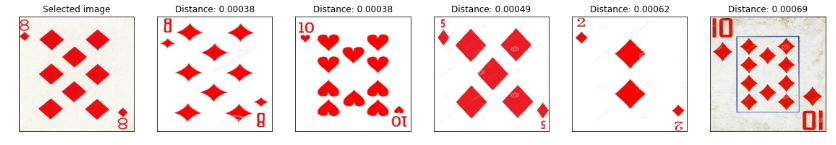
\includegraphics[width=\textwidth]{imgs/comb2.png}
    \end{figure}
    \item Prioritizing the ranking based on the HOG descriptor followed by the top 20 ranked images based on the histogram descriptor.
    \begin{figure}[H]
        \centering
        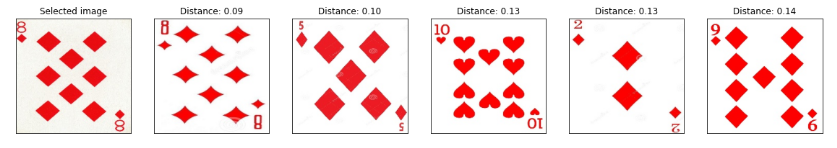
\includegraphics[width=\textwidth]{imgs/comb3.png}
    \end{figure}
\end{itemize}

This way, depending on our priorities, we can select one or another method.

On balance, the implementation of Content-Based Image Retrieval (CBIR) for poker cards in online gaming applications enhances user interaction. The `smart' histogram descriptor, emphasizing color and intensity, refines card recognition. The weighted approach on a $5 \times 4$ grid further fine-tunes this descriptor. The introduction of an additional descriptor, merging Harris corners and Histogram of Oriented Gradients (HOG), enriches the feature set. Experimentation with combination strategies demonstrates the versatility of CBIR. By blending academic insights with practical applications, our project aims to advance efficient re-identification methods for real-world scenarios.


\printbibliography[heading=bibintoc]

\end{document}
